\noindent

\includegraphics[height=1.25cm]{images/pictograms/replication}

\includegraphics[height=1.25cm]{images/pictograms/benchmark}

\includegraphics[height=1.25cm]{images/pictograms/under_construction}

\includegraphics[height=1.25cm]{images/pictograms/pic}

\includegraphics[height=1.25cm]{images/pictograms/nonlinear}

\includegraphics[height=1.25cm]{images/pictograms/paraview}

\includegraphics[height=1.25cm]{images/pictograms/publication}
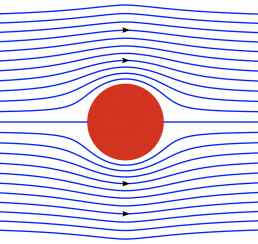
\includegraphics[height=1.25cm]{images/pictograms/streamfunction}


%%%%%%%%%%%%%%%%%%%%%%%%%%%%%%%%%%%%%%%%%%%%%%%%%%%%%%%%%%%%%%%%%%%%%%%%%%%%%%%%%%%%%%%%%%%%%%%%%%%

\begin{flushright} {\tiny {\color{gray} python\_codes/fieldstone\_156/text.tex}} \end{flushright}

%\lstinputlisting[language=bash,basicstyle=\small]{python_codes/template_keywords.key}

\par\noindent\rule{\textwidth}{0.4pt}

\begin{center}
\inpython
{\small Code: \url{https://github.com/cedrict/fieldstone/tree/master/python_codes/fieldstone_156}}
\end{center}

\par\noindent\rule{\textwidth}{0.4pt}

%%%%%%%%%%%%%%%%%%%%%%%%%%%%%%%%%%%%%%%%%%%%%%%%%%%%%%%%%%%%%%%%%%%%%%%%%%%%%%%%%%%%%%%%%%%%%%%%%%%

This \stone is inspired by and is meant to be an incomplete 
replication of \textcite{ketu90}. Most of what follows is copied verbatim from the paper.
The code is mine.

Major goals of this work are to generate a flow in two
dimensions that is chaotic in both space and time and
to calculate the deformation of a strain marker in that flow.
The flow is confined to a box of length $w$ and detph $h$.
The stream function is specified as follows:
\begin{equation}
\Psi = 
\left(
\frac{\lambda \sqrt 2}{\pi^2}
\right)
\sin \pi y'
\left\{
B(t') \sin \frac{\pi x'}{\lambda}
+[C(t')-27]\sin \frac{2 \pi x'}{\lambda}
\right\}
\label{eq:ketupsi}
\end{equation}
where $x'=x/h$, $y'=y/h$, $\lambda=w/h$ and $t'$ is the nondimensional
time. 
$B$ and $C$ are time-dependent driver of the flow. This solution satisfies 
conservation of mass and free slip conditions. 
The flow contains either one or two convection cells within the box,
depending on the magnitude of $B$ and $C$.
As B and C vary smoothly but chaotically in time, the flow will oscillate
smoothly but chaotically between one and two cells. 

The flow is driven using the solutions to the Lorenz equations in the chaotic regime:
\begin{eqnarray}
\frac{\partial A}{\partial t'} &=& -\sigma A + \sigma B \label{eq:Lorenz1}\\ 
\frac{\partial B}{\partial t'} &=& -AC + rA -B \label{eq:Lorenz2}\\ 
\frac{\partial C}{\partial t'} &=& AB - bC \label{eq:Lorenz3}
\end{eqnarray}
where $\sigma$, $r$, and $b$ are parameters and $t'=\pi^2 (1+\lambda^{-2}) \kappa t /h^2$
is the nondimensional time with $b=4/(1+\lambda^{-2})$ and $\kappa$ the thermal diffusivity. 

These are numerically integrated to find the time dependence of the solution. 
The parameters $\sigma$ and $r$ represent the Prandtl number  and the ratio
of the Rayleigh number to the critical Rayleigh number for the onset of convection.

In the study the authors use: $r=28$, $\sigma=10$, and $b=8/3$ ($\lambda=\sqrt 2$).
The solution to this problem has three fixed points, corresponding to
steady flows:

\begin{itemize}
\item $A=B=C=0$ which corresponds to no convection;
\item $A=B=6\sqrt 2$ and $C=27$
\item $A=B=-6\sqrt 2$, $C=27$
\end{itemize}
These steady solutions are unstable, however, and after an initial transient, the solutions 
to the equations above approach the strange attractor in $A-B-C$ space.
The solution spirals around the fixed points $A=B=6\sqrt 2$, $C=27$ and 
$A=B=-6\sqrt 2$, $C=27$. It is however non repeating, and the solution is highly sensitive to the initial 
conditions. 

In the physical $x-y$ space, the flow obtained from Lorenz's
model is chaotic in time but not space; a particle follows
a closed path, corresponding to a single streamline, but
its position on that path and its velocity are chaotic in time.
This is unlikely to occur in real fluids, and the Lorenz model 
has very limited direct applicability to real thermal flows.

The Lorenz model cannot be directly applied to mantle convection, 
because at infinite Prandtl number, the chaotic behavior disappears and the Lorenz 
model reverts to steady convection.




The velocity field is obtained as follows\footnote{The authors use a different 
convention for the minus sign so these velocities are opposites of those in the paper.}:
\begin{eqnarray}
u'(x',y') 
&=& \frac{\partial \Psi}{\partial y'} 
= \left(
\frac{\lambda \sqrt 2}{\pi}
\right)
\cos \pi y'
\left\{
B(t') \sin \frac{\pi x'}{\lambda}
+[C(t')-27]\sin \frac{2 \pi x'}{\lambda}
\right\} \nn\\
v'(x',y') 
&=& -\frac{\partial \Psi}{\partial x'} 
=-
\left(
\frac{ \sqrt 2}{\pi}
\right)
\sin \pi y'
\left\{
B(t') \cos \frac{\pi x'}{\lambda}
+2[C(t')-27]\cos \frac{2 \pi x'}{\lambda}
\right\}
\end{eqnarray}
We can easily verify that $u'(x'=0)=u'(x'=1)=0$ and
$v'(x',y'=0)=v'(x',y'=1)=0$  VERIFY!



The evolution of the flow is shown in the figure here under, 
which contains a projection of the solution of the Lorenz equations 
onto the $B-C$ plane:

\begin{center}
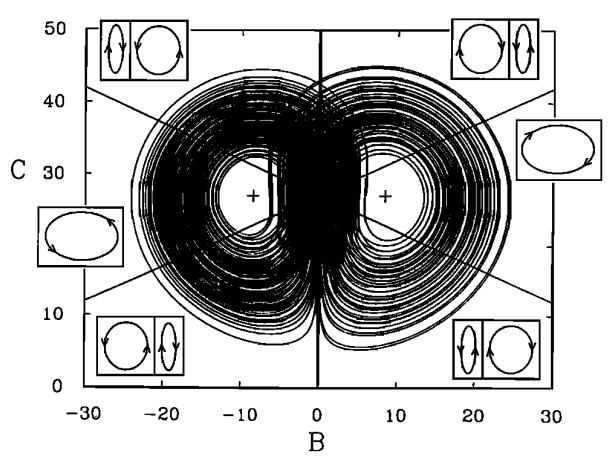
\includegraphics[width=10cm]{python_codes/fieldstone_156/images/ketu90a}\\
{\captionfont Evolution of the Lorenz variables $B$ and $C$,
which govern the time-dependent flow of equation \eqref{eq:ketupsi}.
This is the solution to the Lorenz equations
\eqref{eq:Lorenz1}-\eqref{eq:Lorenz3} projected onto the $B-C$ plane. It is calculated
using  $\sigma$=10, $r$=28, and $b = 8/3$. The inset figures are
schematics of the streamlines of \eqref{eq:ketupsi} corresponding
different values of $B$ and $C$. The flow used in the mixing 
calculations oscillates smoothly between one and two cells.}
\end{center}

The figure is divided into regions corresponding
to the differing flow regimes. The inset figures
show schematically the streamlines obtained for
different values of $B$ and $C$. Though the streamlines
are closed at all times, particle trajectories are not, and
the resulting flow has space-filling particle paths.

A representative particle path is shown in the next figure
after times of $t'=1$ (one overturn time), $t'=10$, and $t'=100$.
The flow is space-filling in that a particle will eventually
migrate to every point in the box. 


\begin{center}
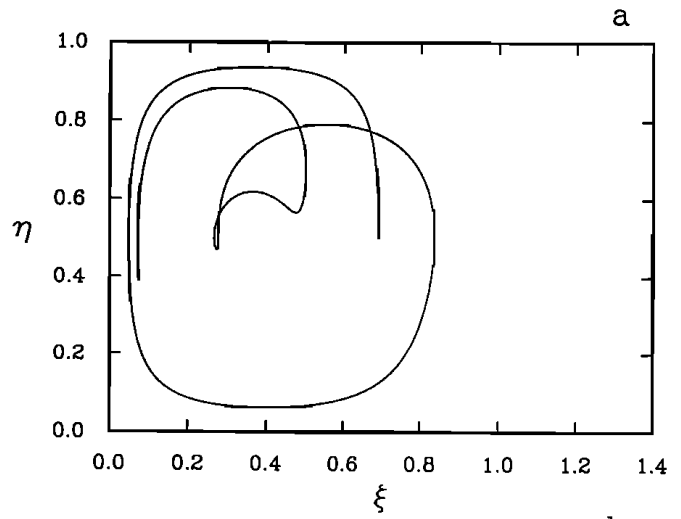
\includegraphics[width=5.7cm]{python_codes/fieldstone_156/images/ketu90b}
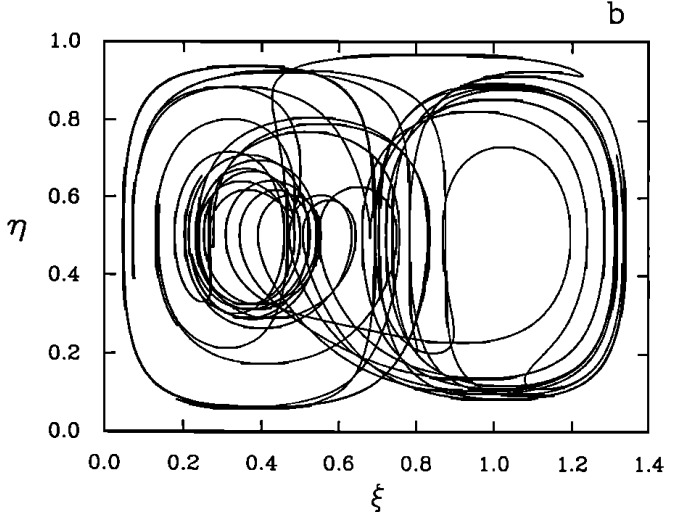
\includegraphics[width=5.7cm]{python_codes/fieldstone_156/images/ketu90c}
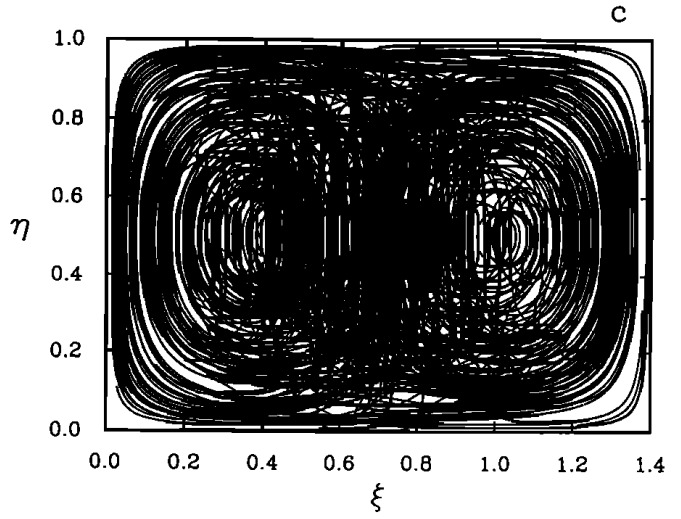
\includegraphics[width=5.7cm]{python_codes/fieldstone_156/images/ketu90d}\\
{\captionfont 
Particle trajectory in the chaotic flow. The particle 
path is shown after times of (a) $t'=1$, (b) $t'=10$, 
and (c) $t'=100$. The particle is initially positioned
at the center of the box.
}
\end{center}


A group of particles
which are initially clustered close together will eventually 
be driven apart and scattered evenly throughout the box:

\begin{center}
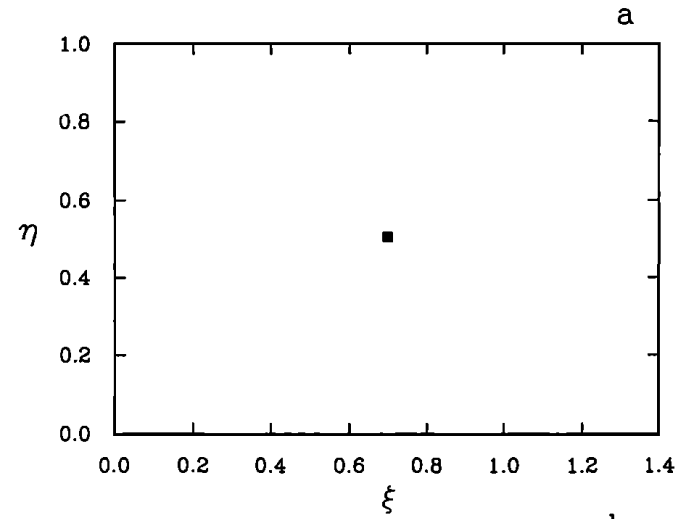
\includegraphics[width=5.7cm]{python_codes/fieldstone_156/images/ketu90e}
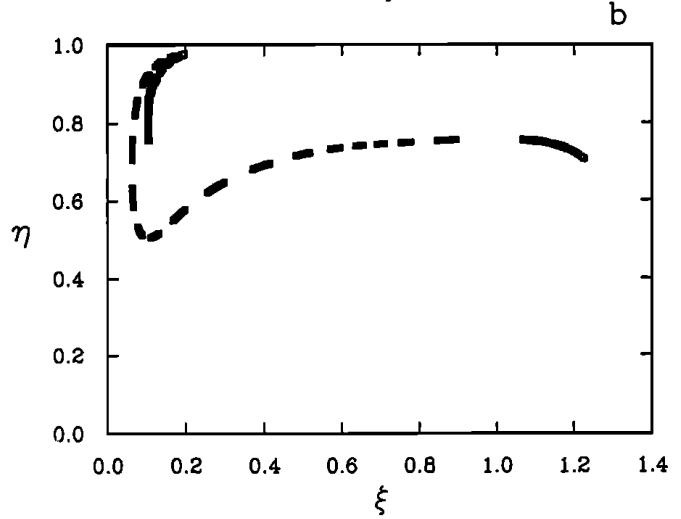
\includegraphics[width=5.7cm]{python_codes/fieldstone_156/images/ketu90f}
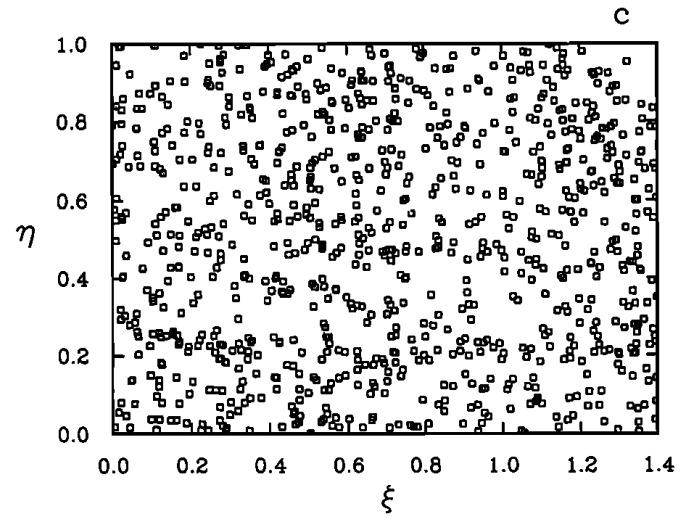
\includegraphics[width=5.7cm]{python_codes/fieldstone_156/images/ketu90g}\\
{
Scattering of a cluster of particles in the chaotic flow.
(a) 900 particles are placed near the center of the box, 
and their positions are tracked and plotted after times 
of (b) $t'=1$ and (c) $t'=10$.
}
\end{center}

%%%%%%%%%%%%%%%%%%%%%%%%%%%%%%%%%%%%%%%%%%%%%%%%%%%%%%%%%%%%%%%%%
\subsection*{Code specifics}


The domain is a rectangle of size $L_x,L_y$ with $L_x=w=\sqrt 2$ and $L_y=h=1$
so that $\lambda=w/h=\sqrt 2$ as in the publication (see figures above).
We set $\sigma=10$, $r=28$ and $b=8/3$. 
What we ultimately miss are the initial values for $A,B,C$. We cannot start
with all three equal to zero, otherwise we obtain the solution $A=B=C=0$ solution.
Looking at the first figure in $B-C$ space we see that the values are constrained in 
$[-30,30]\times[0,50]$ so we can set $B=0.5$ and $C=25$ at $t'=0$. 
For now we also set $A=0$ at startup. 

At the moment markers are set on a 40x40 grid in a square of size 0.025x0.025
placed in the middle of the domain, and they are advected by means of a simple Euler step. 


The code then must solve Eqs.~\eqref{eq:Lorenz1},\eqref{eq:Lorenz2},\eqref{eq:Lorenz3}.
These are coupled first-order nonlinear equations. This is no good news and 
specific numerical techniques should be used in this case. 
To get things started I nevertheless opt for a simplistic approach. 
The time derivatives are discretised by means of 1st order explicit formulas ({\tt scheme 1}):
\begin{eqnarray}
\frac{A^{n+1}-A^n}{\delta t} &=& -\sigma A^n + \sigma B^n \\
\frac{B^{n+1}-B^n}{\delta t} &=& -A^n C^n + rA^n -B^n  \\
\frac{C^{n+1}-C^n}{\delta t} &=& A^n B^n - bC^n \label{eq:Lorenz3}
\end{eqnarray}
where the upperscript denotes the timestep. We will use tiny time steps and hope for the best.

Every time that new $B$ and $C$ values are obtained we can use these to compute the 
velocity field and to drive the flow.


\begin{center}
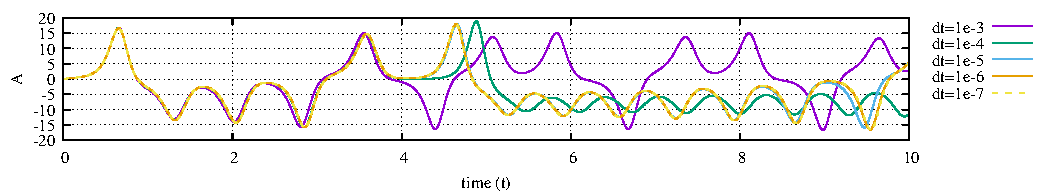
\includegraphics[width=5.7cm]{python_codes/fieldstone_156/results/scheme1/A.pdf}
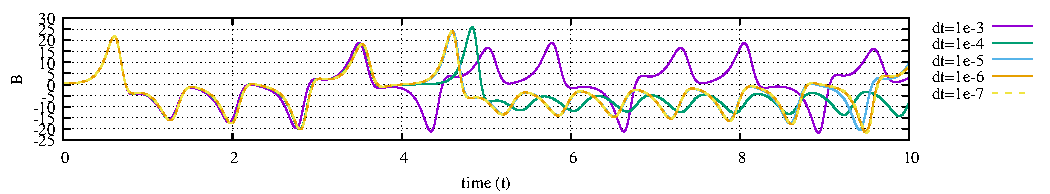
\includegraphics[width=5.7cm]{python_codes/fieldstone_156/results/scheme1/B.pdf}
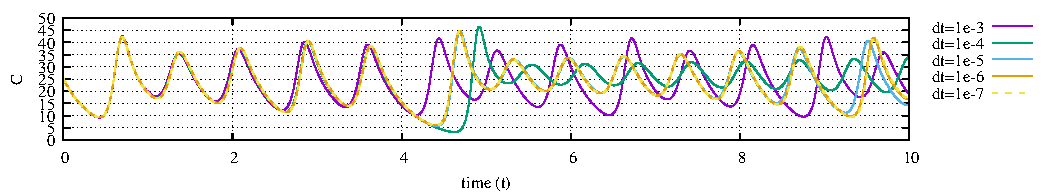
\includegraphics[width=5.7cm]{python_codes/fieldstone_156/results/scheme1/C.pdf}\\
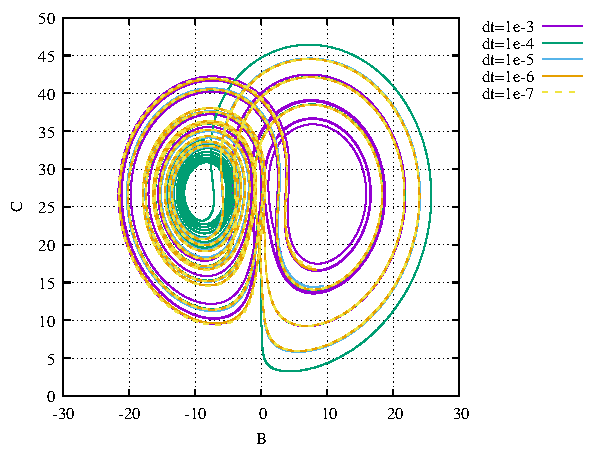
\includegraphics[width=9cm]{python_codes/fieldstone_156/results/scheme1/BC.pdf}\\
{\captionfont Given the simplistic integration scheme, we find that 
even using very small time steps results diverge after $t'=10$.}
\end{center}

Based on these encouraging results, it is now time to look at a more appropriate
scheme to solve the equations.

We can try something very simple, i.e. use updated values of $B$ and $C$ when possible ({\tt scheme 2}):
\begin{eqnarray}
\frac{A^{n+1}-A^n}{\delta t} &=& -\sigma A^n + \sigma B^n \\
\frac{B^{n+1}-B^n}{\delta t} &=& -A^{n+1} C^n + rA^{n+1} -B^n  \\
\frac{C^{n+1}-C^n}{\delta t} &=& A^{n+1} B^{n+1} - bC^n \label{eq:Lorenz3}
\end{eqnarray}
i.e.
\begin{eqnarray}
A^{n+1} &=& (-\sigma A^n + \sigma B^n) \delta t + A^n \\
B^{n+1} &=& (-A^{n+1} C^n + rA^{n+1} -B^n ) \delta t+ B^n \\
C^{n+1} &=& (A^{n+1} B^{n+1} - bC^n ) \delta t + C^n
\end{eqnarray}

\begin{center}
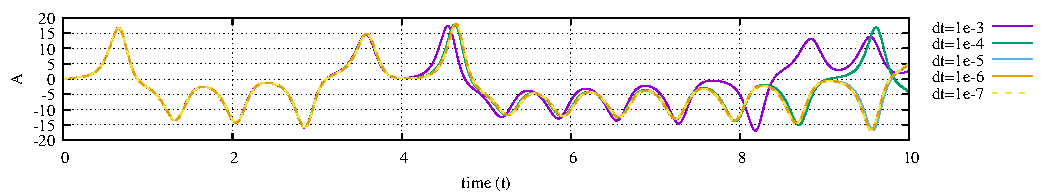
\includegraphics[width=5.7cm]{python_codes/fieldstone_156/results/scheme2/A.pdf}
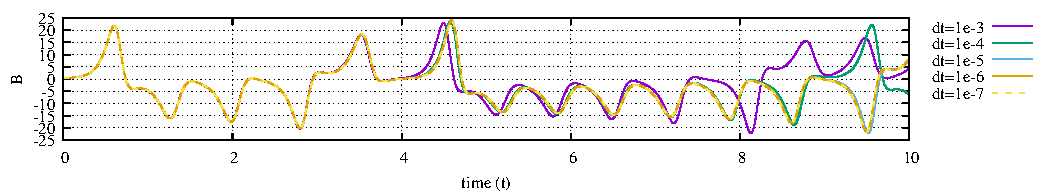
\includegraphics[width=5.7cm]{python_codes/fieldstone_156/results/scheme2/B.pdf}
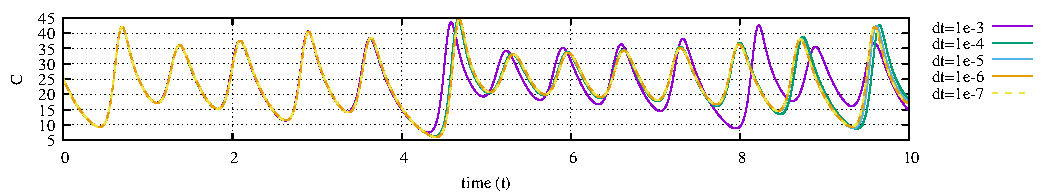
\includegraphics[width=5.7cm]{python_codes/fieldstone_156/results/scheme2/C.pdf}\\
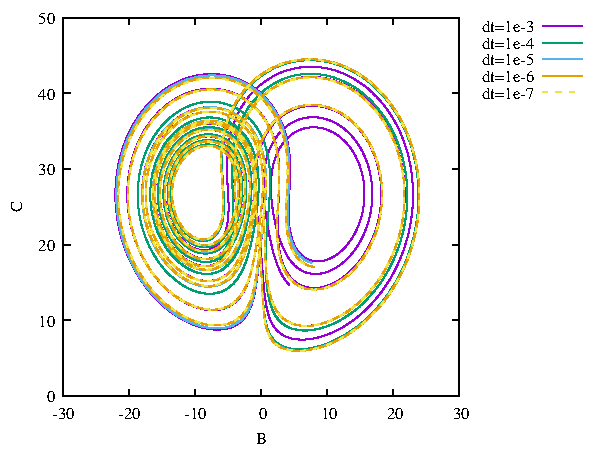
\includegraphics[width=9cm]{python_codes/fieldstone_156/results/scheme2/BC.pdf}\\
\end{center}

This is somewhat better, lines with 'large' $\delta t$ are closer to the reference
$\delta t=5\cdot 10^{-5}$ line. 

\url{https://www.youtube.com/watch?v=Bd9rRSSbH1o}


\begin{center}
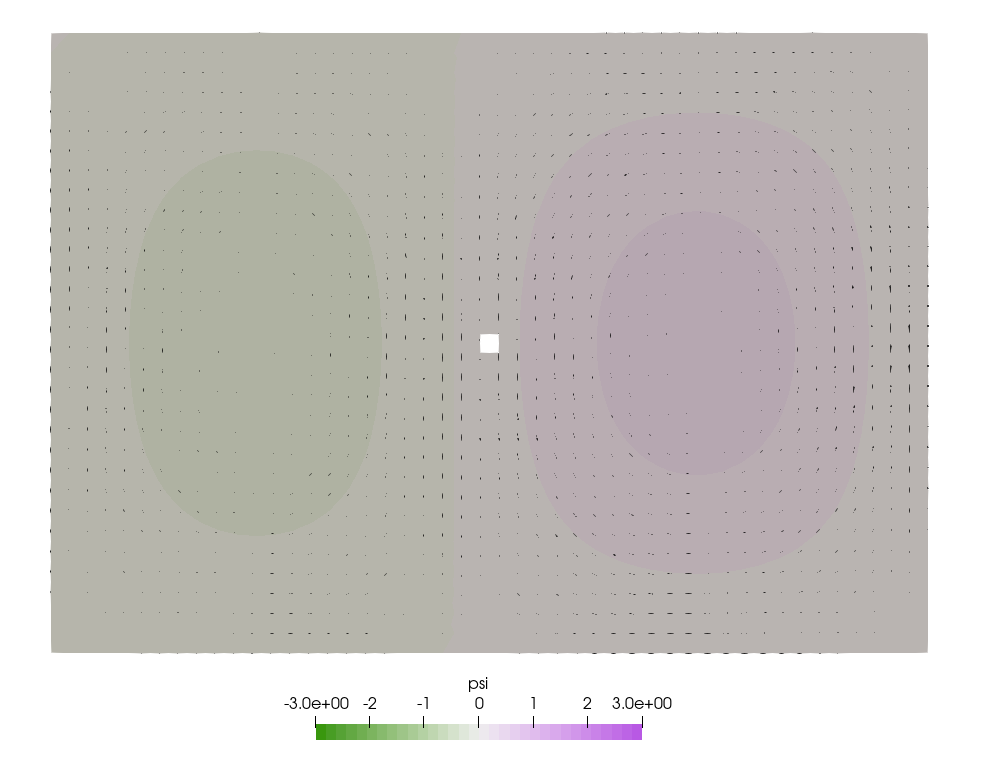
\includegraphics[width=5.7cm]{python_codes/fieldstone_156/results/scheme2/psi0000}
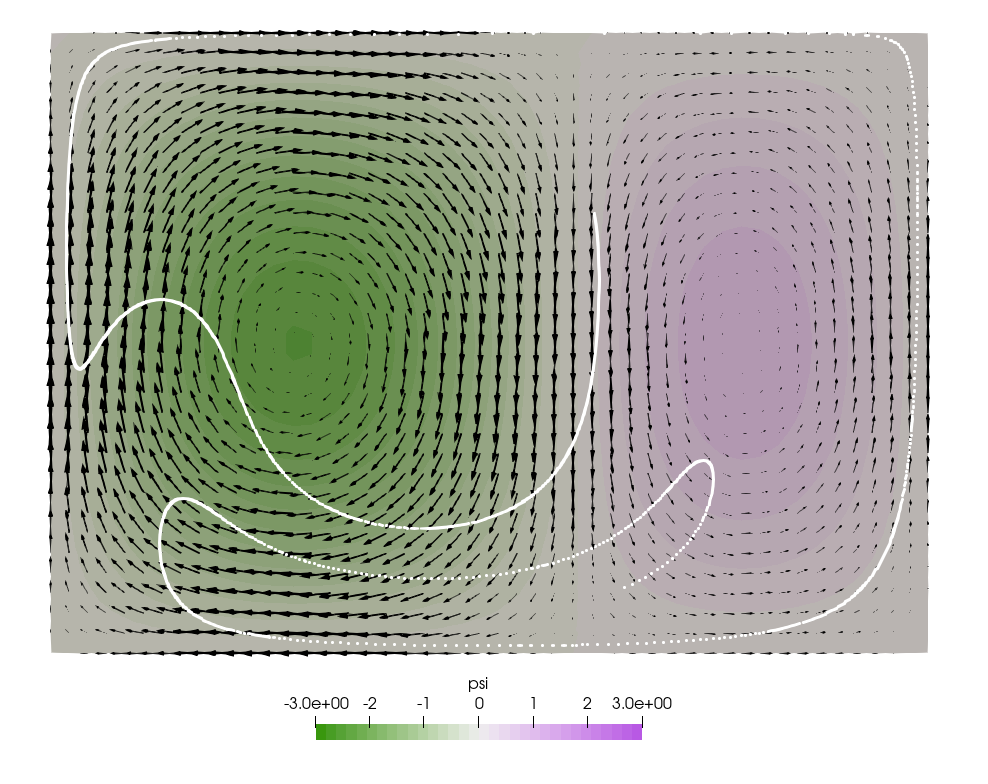
\includegraphics[width=5.7cm]{python_codes/fieldstone_156/results/scheme2/psi0100}\\
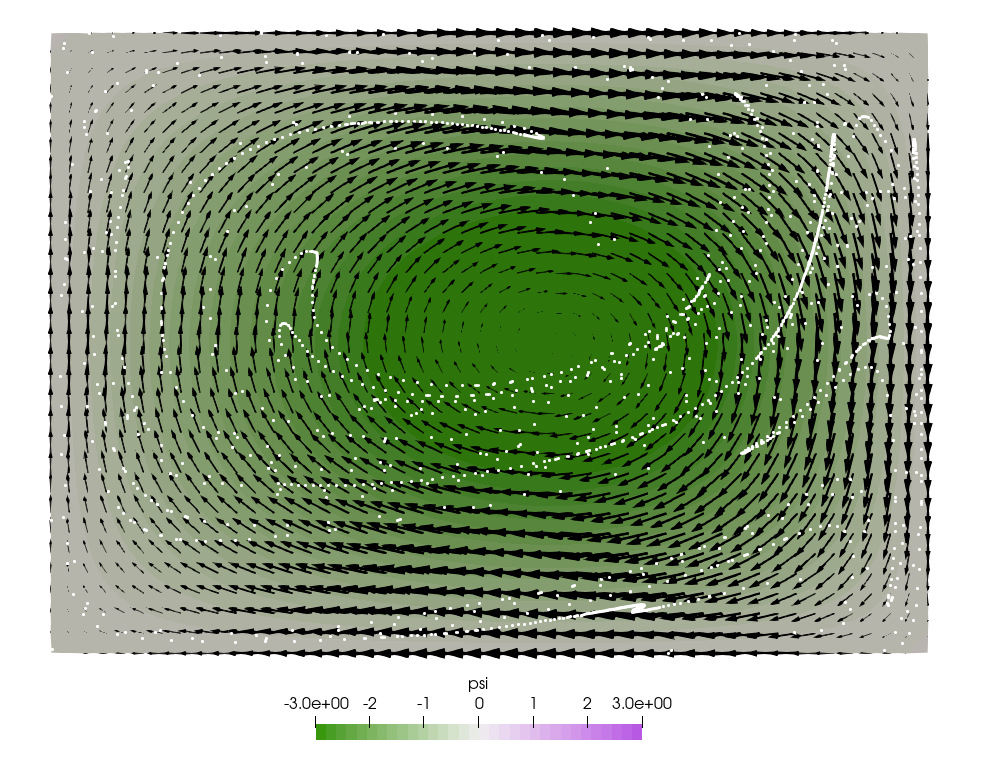
\includegraphics[width=5.7cm]{python_codes/fieldstone_156/results/scheme2/psi0200}
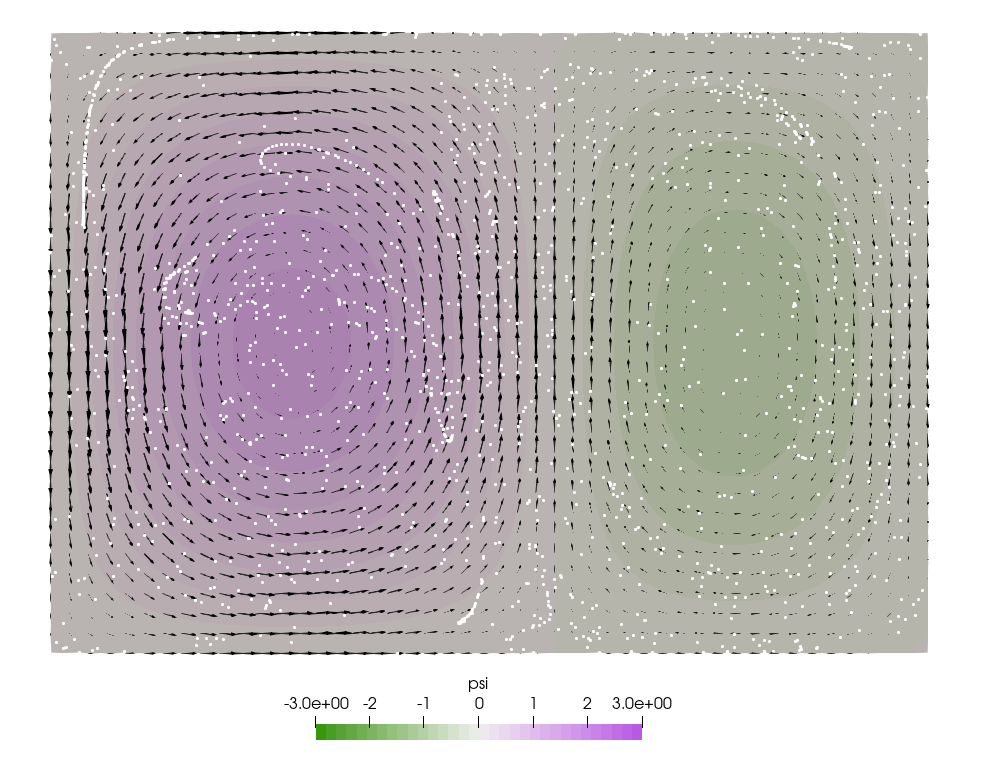
\includegraphics[width=5.7cm]{python_codes/fieldstone_156/results/scheme2/psi0300}\\
{\captionfont Markers, stream function field and velocity arrows. Obtained with $\delta t=10^{-4}$.}
\end{center}

Scheme 3 does iterations at each time step:

\begin{center}
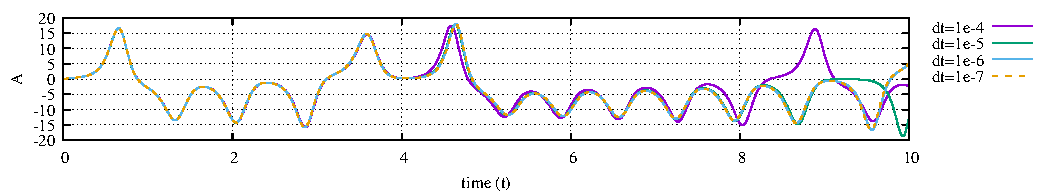
\includegraphics[width=5.7cm]{python_codes/fieldstone_156/results/scheme3/A.pdf}
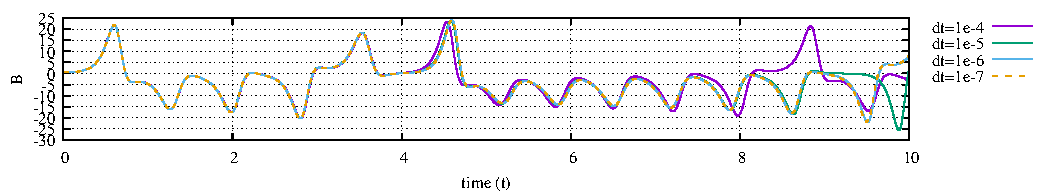
\includegraphics[width=5.7cm]{python_codes/fieldstone_156/results/scheme3/B.pdf}
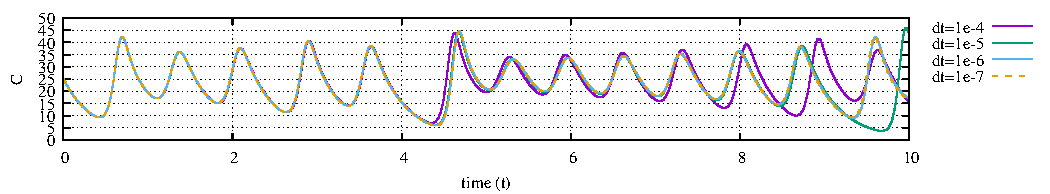
\includegraphics[width=5.7cm]{python_codes/fieldstone_156/results/scheme3/C.pdf}\\
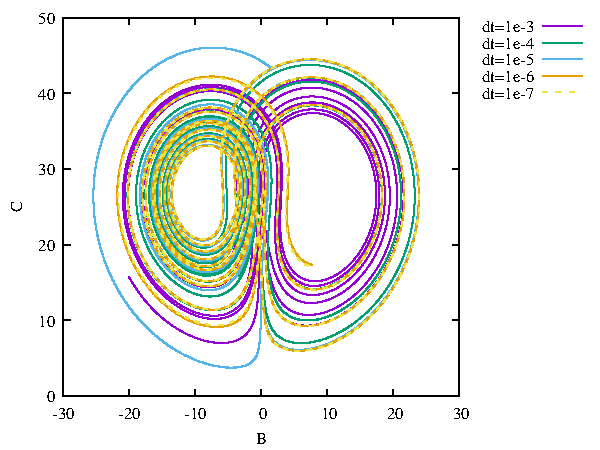
\includegraphics[width=9cm]{python_codes/fieldstone_156/results/scheme3/BC.pdf}\\
{\captionfont Not sure what to make of it... looks different than the other two...}
\end{center}



%%%%%%%%%%%%%%%%%%%%%%%%%%%%%%%%%%%%%%%%%%%%%%%%%%%%%%%%%%%%%%%%%%%%%%%%%%%%%%%%%%%%%%%%%%%%%%%%%%%
\par\noindent\rule{\textwidth}{0.4pt}

\vspace{.5cm}

\begin{center}
\fbox{\begin{minipage}{0.9\textwidth}
{\color{teal}To Do, open questions, future work?}
\begin{itemize}
\item export ABC only at steps of 0.01 for lighter files
\item implement high accuracy scheme for PDEs integration
\item implement high accuracy for markers advection
\end{itemize}
\end{minipage}}
\end{center}



